%%%%%%%%%%%%%%%%%%%%%%%%%%%%%%%%%%%%%%%%%%%%%%%%%%%%%%%%%%%%%%%%%%% 
%                                                                 %
%                            CHAPTER                              %
%                                                                 %
%%%%%%%%%%%%%%%%%%%%%%%%%%%%%%%%%%%%%%%%%%%%%%%%%%%%%%%%%%%%%%%%%%% 
%\chapter{Structuur van de masterproeftekst}
\chapter{Herkenning en Detectie Algemeen}

\section{Deep learning-gebaseerde herkeningssystemen}
Herkeningssytemen systemen voorspellen wat de klasse van een object is in een afbeelding. 
Dus het herkennen van objecten in digitale afbeeldingen zonder deze te lokaliseren of aan te duiden. 
Bij herkeningssystemen is er geen of weinig overlap tussen de trainingsafbeeldingen en de inputafbeeldingen.
Bijvoorbeeld bij een gezichts herkenningssysteem wordt er een algemeen herkeningssystemen ontworpen dat gezichten herkent, en niet elk individueel gezicht herkent.
Voor een herkenningssysteem is er een goed getraind netwerk nodig dat input afbeeldingen omzet in features. 
Er moet een database zijn met daarin de gegevens van de objecten die men wilt herkennen. 
Vervolgens hebben is er ook een methode nodig om features van het neuraal netwerk te vergelijken met de gegevens in de database om het juiste object te herkennen.

\subsection{Herkenning}
Eens dat er een getraind CNN is kunnen we verdergaan met de effectieve herkenning. 
Als men bepaald objecten in een afbeelding wil ontdekken gaat men met behulp van het CNN de afbeelding omzetten in een embedding. 
Embeddings zijn vector representaties die kunnen worden vergeleken in een embedding space, waar gelijkaardige objecten dichter bij elkaar liggen. De embedding van de input afbeelding wordt vergeleken met de embeddings die zich in een gallerij bevinden. 
De gallerij is een database/verzameling met gekende embeddings/ID's van de objecten die men wilt herkennen.
Met behulp van een query kunnen we gelijkaardige objecten uit de gallerij halen om deze te gaan vergelijken in een embedding space. 
Een query is een embedding van de input waarvan het label niet gekend is.
Gelijkaardige embeddings kunnen gezocht worden via de nearest neighbour techniek, waar we naar de klasse van de dichtsbijzijnde buur gaan kijken.

%meer uitleg over embedding space en nearest neighbour techniek

\subsection{convolutioneel neuraal netwerk (CNN) }
\begin{figure}[!ht]
    \centering
 	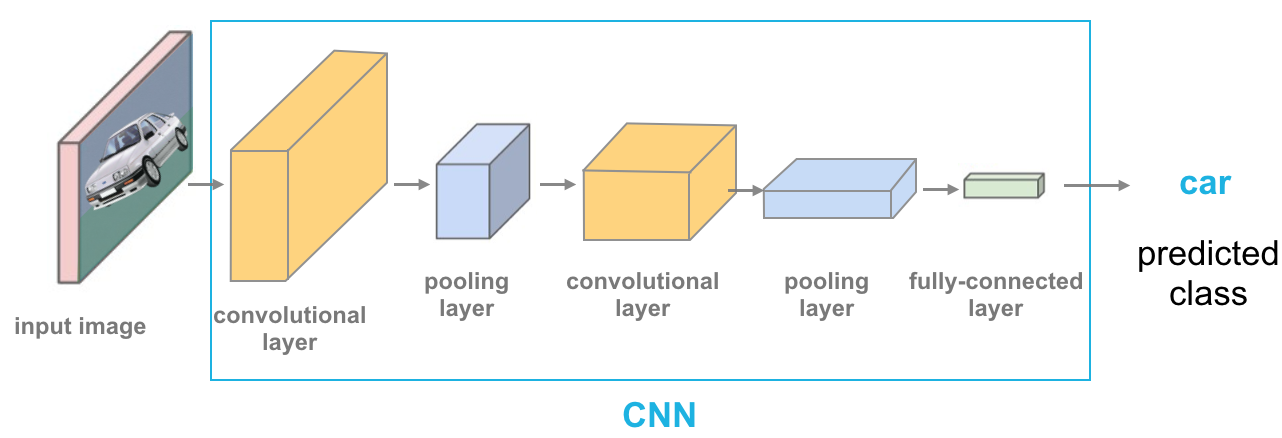
\includegraphics[width=0.80\linewidth]{fig/CNN.png}
 	\caption{CNN met 2 convolutie lagen en 2 pooling lagen en een fully-connected layer}
 	\label{fig:cnn}
\end{figure}

De belankrijkste bouwsteen van een herkenningssysteem is een goed getrainde CNN (figuur \ref{fig:cnn}). 
In tegenstelling tot fully connected netwerken wordt bij een CNN de gewichten gedeeld over verschillende locaties om zo het aantal parameters te verminderen.
 
Het belangrijkste deel van een CNN zijn de convolutielagen (figuur \ref{fig:conv_laag}) waarbij men een kernel/filter over de input laat gaan wat als output een feature map genereerd. 
Een kernel bestaat uit set van gewichten die met de input worden vermenigvuldigd, deze kernel wordt over de input afbeelding geschoven. 
Al de pixels binnen het veld van de kernel worden gereduceert tot een enkele waarde. 
CNN leren verschillende features met verschillende kernels in parallel. 
Waardoor de matrices met feature mappen steeds kleiner worden maar ook dieper worden. Een andere factor van een convolutie laag is de stride, deze waarde geeft aan met hoeveel pixels de kernel telkens moet doorschuiven. 
Een CNN bestaat uit een opeenvolging van een aantal convolutie lagen die steeds meer high-level features extraheren. Hoe meer convolutielagen een netwerk telt hoe meer features er uit de input worden gehaald, maar hoe trager het netwerk is. 

\begin{figure}[!ht]
	\centering
	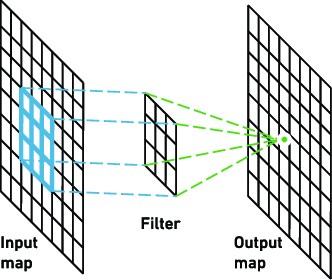
\includegraphics[width=0.35\linewidth]{fig/convolution layer.png}
	\caption{Convolutie laag waarbij een filter wordt herleid tot een output feature.}
	\label{fig:conv_laag}
\end{figure}

Elke convolutie laag wordt gevolgd door een niet-lineare activatie functie, de meest gebruikt functie hiervoor is de rectified linear unit (ReLu) (figuur \ref{fig:relu}). 
De ReLu wordt vaak gebruikt omdat deze eenvoudig is, kan exact 0 weergeven en ziet er lineair uit. 
Max(0,x) is de ReLu bewerking, dus er wordt verdergegaan met 0 of de input waarde. 
Zonder een niet-lineare activatie functie kan het CNN herleid worden tot 1 convolultie laag die geen high-level features kan extraheren. 
Andere mogelijkheden voor Lineare activatie functies zijn: Sigmoid en Tangens hyperbolicus maar deze functies vragen meer rekenwerk.

\begin{figure}[!ht]
 	\centering
 	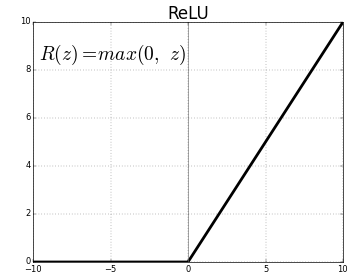
\includegraphics[width=0.35\linewidth]{fig/ReLu.png}
 	\caption{ReLu, waarbij het maximum wordt genomen van 0 en de input waarde.}
 	\label{fig:relu}
\end{figure}

Een volgende bouwsteen is de pooling laag waarbij het aantal samples in de feature map wordt verlaagt. 
De meest voorkomende methode is max-pooling waarbij er verder wordt gegaan met de maximum waarde in een bepaalde regio. 
Het doel van een pooling laag is om het aantal parameters te verminderen en zo ook het rekenwerk te verminderen. 
Er kan ook gebruik gemaakt worden van avarage pooling waarbij er verder wordt gegaan met de gemiddelde waarde van een regio. 
Er is ook minimal pooling waarbij er verder wordt gegaan met de minimum waarde.

Op het einde van elk CNN volgen er meestal 1 of meerdere fully connected lagen. 
Deze lagen connecteren elke input van \'e\'en laag met elke activatie eenheid van de volgende laag. 
Dit zorgt voor meer parameters en meer rekenwerk waardoor deze lagen een vertragende factor vormen. 
De fully connected lagen gaan niet-lineare combinaties leren van de features van de convolutie lagen. 
De fully connected lagen zorgen voor een classificatie op basis van de features van de convolutie lagen.

\subsection{Trainen van een CNN}
Het trainen van een CNN bestaat uit het leveren van veel voorbeelden aan het netwerk. 
Op basis van het resultaat van deze voorbeelden worden telkens de gewichten van de kernels aangepast, zodat er steeds een beter resultaat wordt geleverd. 

De loss functie geeft de error van de voorspelling weer tijdens het trainen van een neuraal netwerk. 
Op basis van de loss functie gaat men via de stochastic gradi\"ent decent de gewichten van het netwerken bijstellen zodat bij een volgende trainingsinput de loss functie een beter resultaat geeft. 
Bij de stochastic gradi\"ent decent wordt er per batch/group trainingsvoorbeelden de gewichten bijgesteld. 
De gradienten worden berekend door de loss af te leiden naar de gewichten via de ketting regel, en de gewichten worden bijgesteld volgens de tegengestelde gradient. 

De learning rate bij het trainen van een CNN be\"invloed de grootte van de stap waarmee de gewichten worden bijgesteld.
Hoe kleiner de learning rate hoe langer het trainen van een CNN duurt.
Maar als de learning rate te hoog is kan het resultaat een slecht getraind netwerk zijn, omdat de veranderingen op de gewichten te groot is om een beter resultaat te verkrijgen.
%kan nog verder worden uitgebreid met back propagation, Loss, epochs, ...

%embeddings worden getraind met triplet loss of autoencoder
%\subsubsection{Triplet loss}

\section{Deep learning-gebaseerde detector}
Object detectie is het lokaliseren en classificeren van objecten in een afbeelding, waarbij de objecten aangeduid worden met een Bounding box. 
Door gebruik te maken van CNN kunnen er vrij nauwkeurige object detectoren ontworpen worden. 
Object detectie maakt voornamelijk gebruik van twee methodes: de single-stage detector en de two-stage detector.

\subsection{Two-stage detector}
Zoals de naam zegt bestaat deze methode uit 2 niveaus. 
het eerste deel worden er Regions of Intrest (RoIs) gecre\"eerd, dit is het filteren van regio's waarbij de kans groot is dat deze een object bevatten. 
Het tweede deel classificeert en verfijnt de lokalisatie van de RoIs die in het eerste deel gecre\"eerd werden. 
Dit gebeurt door elk van de RoIs door een CNN te voeren. 
Region-based Convolutional Neural Network (R-CNN) is het basis principe van de two-stage detectoren weergegeven in figuur \ref{fig:r-cnn}. 
Hierbij wordt met een region proposal algoritme regio's uit de afbeelding gefilterd waar de kans groot is dat er objecten op staan.
R-CNN bestaat uit 3 stappen:
 
\begin{enumerate}
    \item Via een selective search algoritme worden er ongeveer 2000 mogelijke regio's met objecten geselecteerd.
    %selective search ref
    \item Elke mogelijke regio wordt omgezet naar een feature vector via een CNN.
    \item Elke regio wordt vervolgens geclassificeerd met een klas-specifieke SVMs.
\end{enumerate}

\begin{figure}[!ht]
	\centering
	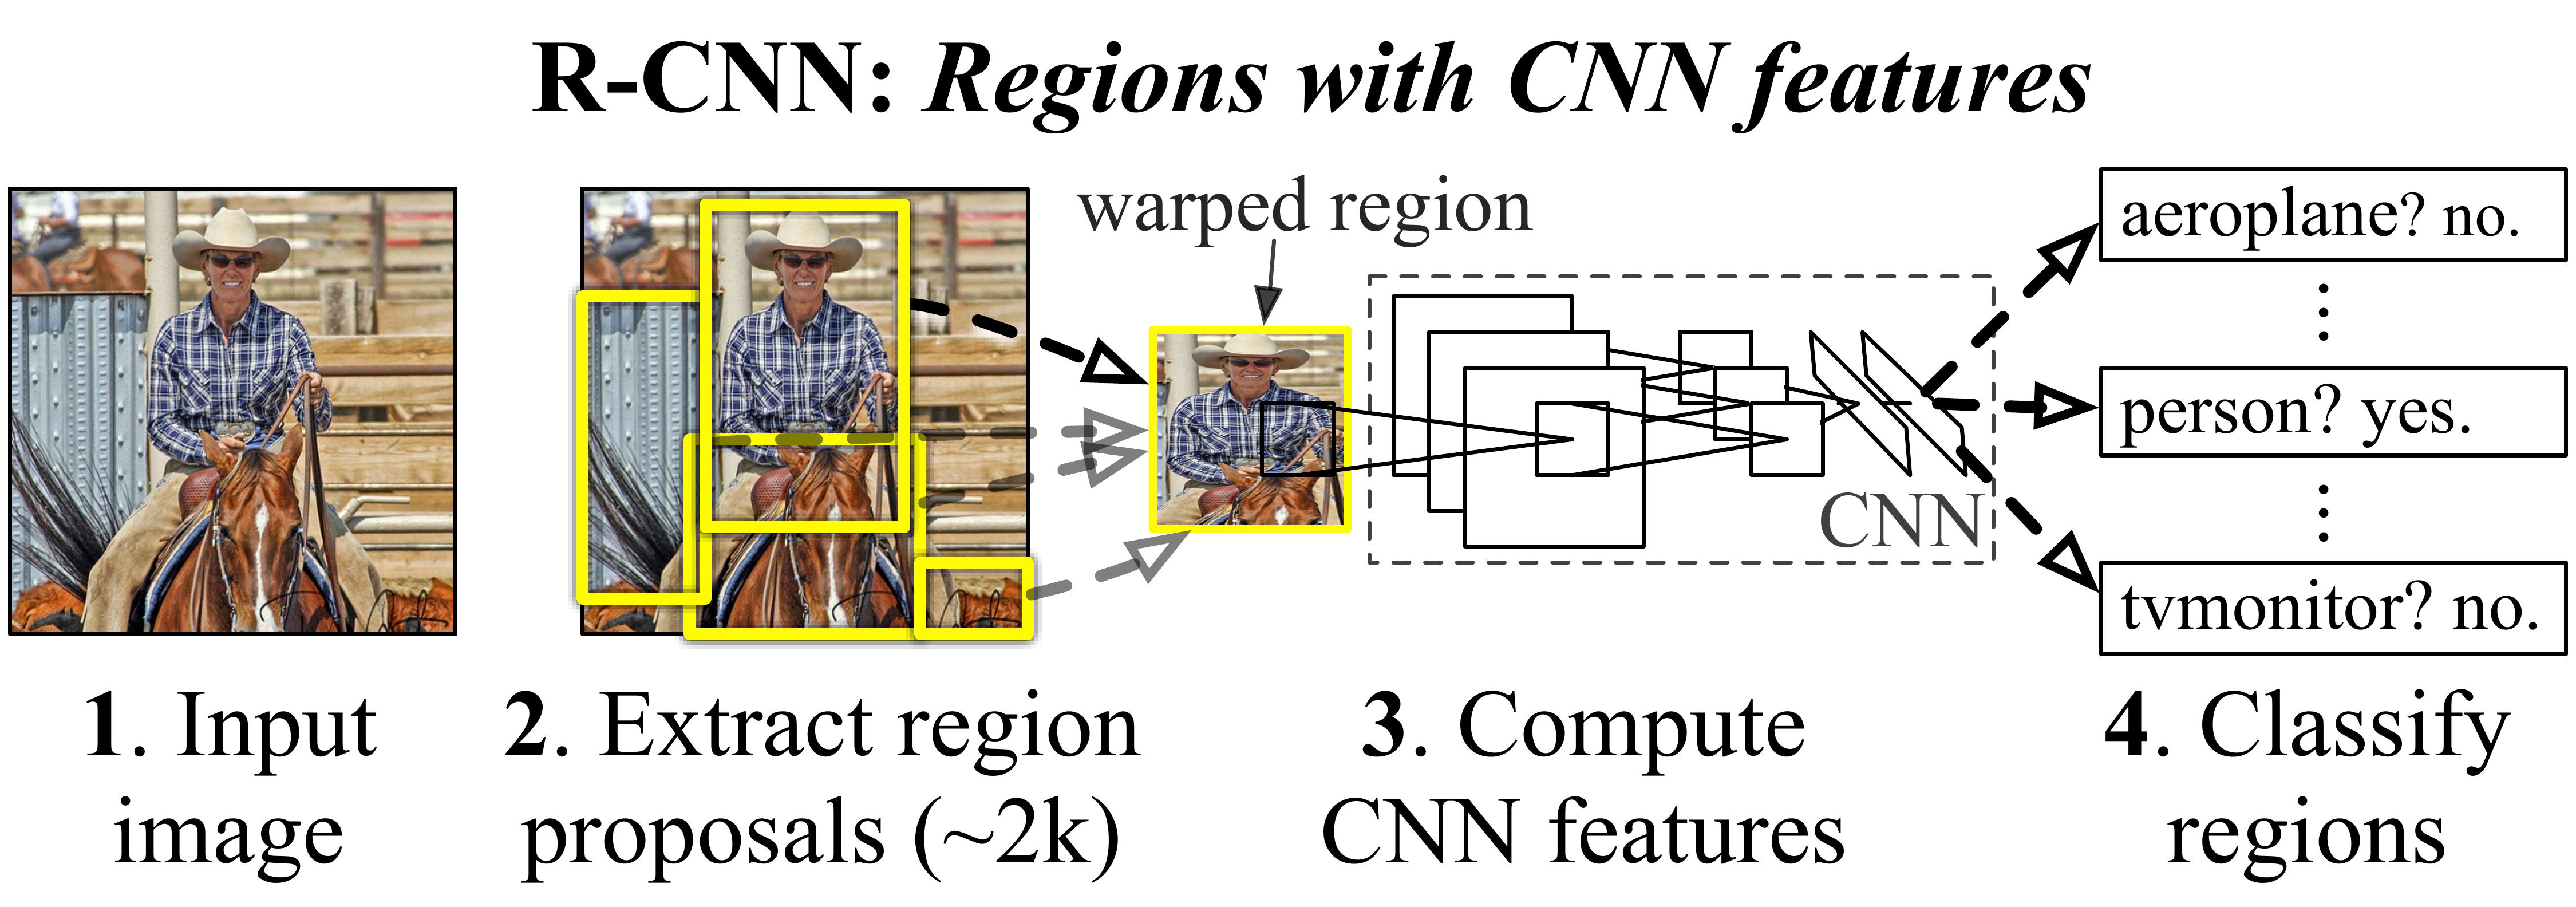
\includegraphics[width=0.70\linewidth]{fig/R-CNN.jpg}
	\caption{R-CNN}
	\label{fig:r-cnn}
\end{figure}

R-CNN is een trage detector vermits elke RoIs door een CNN moet gaan. 
Deze methode is ge\"evolueerd tot de veel snellere methode Faster R-CNN (figuur \ref{fig:faster-r-cnn}). 
Hierbij wordt de afbeelding door een CNN behandelt en vervolgens maakt men gebruik van een Region Proposal Network (RPN). 
Het RPN gaat zoals bij R-CNN regio's uit de afbeelding filteren waar de kans groot is dat er objecten opstaan.
Maar het RPN werkt sneller en levert betere resultaten dan het region proposal algoritme. 

Het RPN is een deep fully convolutional network dat per input een set van regio's als output geeft.
Elk van deze regio's heeft een objectness score wat een maat is voor het object t.o.v. de achtergrond in de afbeelding.
Om een region proposal te genereren wordt het RPN over de feature map geschoven die gegenereerd is door het voorgaande CNN.
Op elke sliding window locatie worden er meerdere regio voorspellingen gedaan.
Deze voorspelling wordt gedaan door verschillende anchor boxen in de sliding window te evalueren.

Vervolgens worden RoIs omgezet naar een feature vector met vaste lengte door RoI pooling.
Elk van deze features gaat door een set van fully-connected lagen die 2 lagen als output heeft.
een softmax laag die de klasse voorspelt, en een bounding box regressie laag die de bounding box voorspelt.
%dieper ingaan op softmax en bbox voorspelling

\begin{figure}[!ht]
    \centering
 	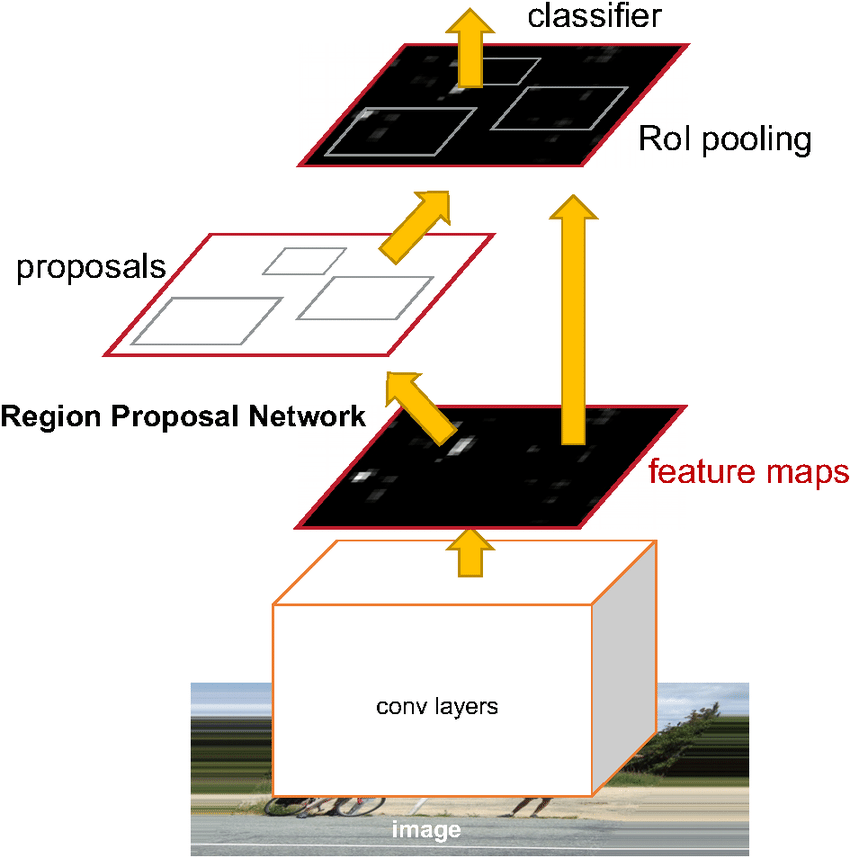
\includegraphics[width=0.3\linewidth]{fig/Faster-R-CNN.png}
 	\caption{Faster R-CNN}
 	\label{fig:faster-r-cnn}
\end{figure}

\subsection{One-stage detector}
Bij one-stage detectoren gebeurt object detectie in \'e\'en keer met \'e\'en neuraal netwerk. 
Dus er is geen region proposal niveau meer zoals bij de two-stage detector. 
Deze detector gebruiken minder geheugen en rekenkracht t.o.v. two-stage detectoren.
One-stage detectoren zijn sneller dan two-stage detectoren omdat ze alles in \'e\'en keer doen, maar kunnen wat in nauwkeurigheid verliezen t.o.v. two-stage detectroren.
De twee meest gebruikte technieken van one-stage detectie zijn: You Only Look Once (YOLO) en Single Shot Detection (SSD).

\begin{figure}[!ht]
	\centering
	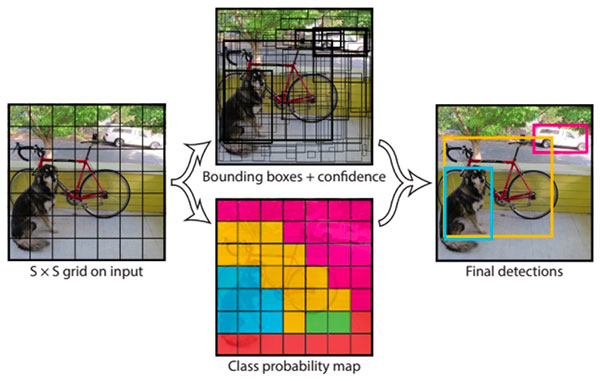
\includegraphics[width=0.60\linewidth]{fig/YOLO.jpg}
	\caption{YOLO waarbij de input is opgedeeld in een S x S rooster. 
	En waarbij bounding box voorspellingen zijn gedaan.}
	\label{fig:yolo}
\end{figure}

YOLO verdeelt de afbeelding in een S x S rooster (figuur \ref{fig:yolo}). 
De cel waarin het middelpunt van het object valt is verantwoordelijk voor de object detectie.
Elke cel voorspelt K aantal bounding boxes en een score die aangeeft hoe zeker het model is dat een bepaalde bounding box een object bevat.
deze score wordt bepaalt met de Intersection Of Union (IOU) tussen de voorspelde box en de ground truth box.
%IOU
Vervolgens is er nog een methode nodig voor de overbodige bounding boxen te verwijderen. 
Een eerste mogelijkheid is door enkel bounding boxen te tekenen waarvan de voorspelling boven een treshold ligt. 
Een andere methode is non-maxima supression deze methode zorgt ervoor dat elk object maar \'e\'en bounding box heeft. 
Deze techniek houdt enkel de bounding box over met de beste voorspelling en onderdrukt de rest van de bounding boxen. 

SSD is een one-stage detector (figuur \ref{fig:ssd}) waarbij een afbeelding door verschillende convolutielagen gaat, wat als resultaat feature mappen op verschillende schalen oplevert.
Op elke locatie van deze feature mappen van verschillende schalen wordt een vaste set van bounding boxen ge\"evalueerd.
Voor elk van deze boxen wordt de zekerheid dat het een object bevat voorspelt.
Op het einde wordt non maximum suppression gebruikt om de finale voorspelling te maken.
Het netwerk van een SSD bestaat uit een basis netwerk dat gevormd wordt door een standaard classificatie netwerk zonder de fully-connected lagen.
Vervolgens worden er extra convolutie lagen toegevoegd, wat het model toelaat om voorspellingen te doen op verschillende schalen.

\begin{figure}[!ht]
	\centering
	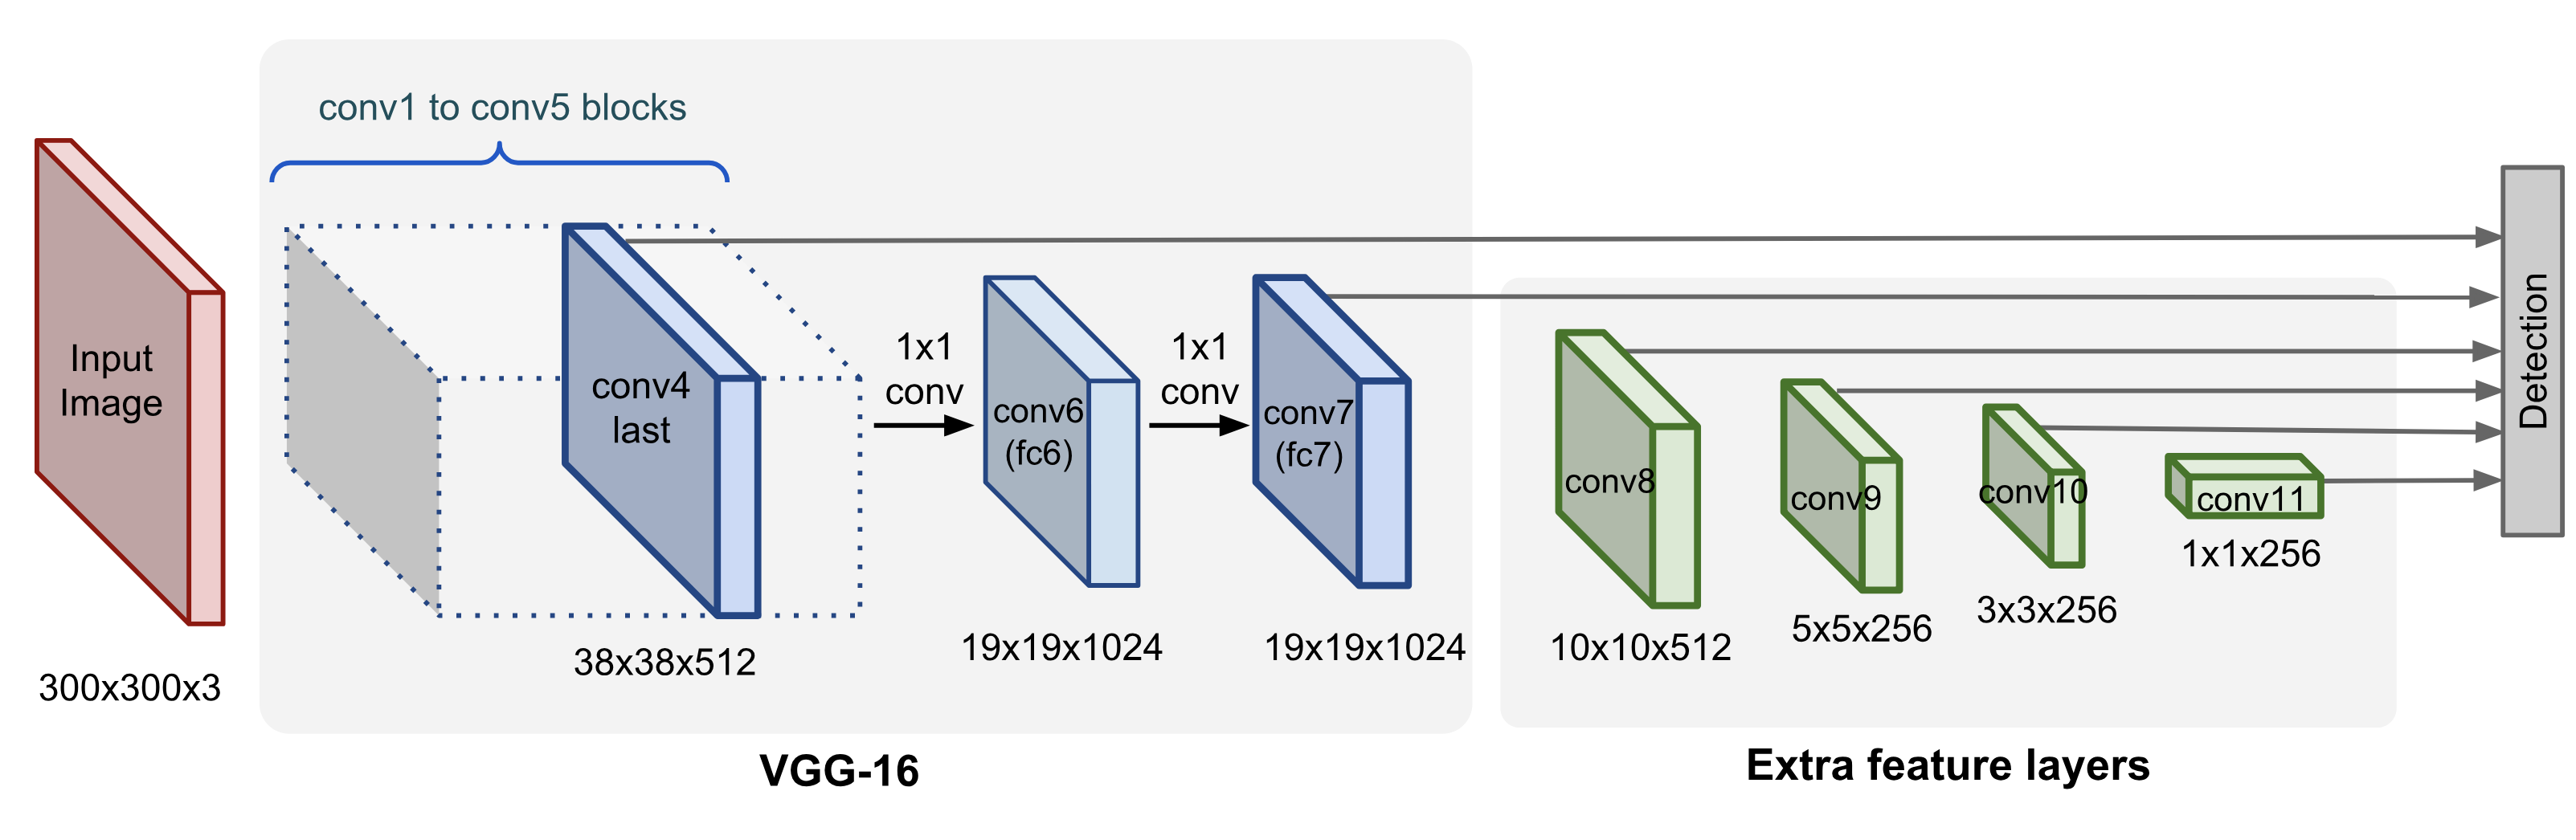
\includegraphics[width=0.80\linewidth]{fig/SSD.png}
	\caption{One-stage detector met VGG net backbone}
	\label{fig:ssd}
\end{figure}

\chapter{Herkenning en detectie implementatie op mobiel platform}

Dit hoofdstuk zal gaan over het implementeren van deep learning herkeningssystemen en detectiesystemen op een mobiel platform.
Hierbij zal het trainen van het CNN model nog steeds gebeuren op een computer.
Bij het uitvoeren van een neuraal netwerk op een mobiel apparaat zal moet men rekening houden met de volgende zaken: 
gelimiteerde rekenkracht, met de batterij en beschikbaar geheugen.
In dit hoofdstuk zullen we een aantal state-of-the-art CNN architecturen voor mobiele platformen bespreken.

\section{Implementatie op mobiele platformen}
Voor de implementatie van neurale netwerken op een mobiel platform kan er gebruik gemaakt worden van een framework.
Deze frameworken zijn een set van tools die de programeur helpen om een machine learning model te implementeren op een mobiel toestel.
De twee meest gebruikte frameworks voor mobiele implementaties zijn: TenserflowLite en Pytorch mobiel.

Tenserflow is ontworpen door Google en is een open source library voor machine learning implementaties.
Door de introductie van de Keras API is Tenserflow gebruiksvriendelijk geworden.
Zo heeft Tenserflow een gebruiksvriendelijk API voor eenvoudige projecten en meer uitgebreide tools voor complexe projecten.
Zo is het met Tenserflow mogelijk om overzichtelijke en elegante code te schrijven.
%Tenserflow kan  dynamisch zijn grafieken wanneer variabelen worden gedeclareerd.
Door gebruik te maken van TensorBoard kan data op een flexibele manier gevisualiseerd worden. 
Tenserflow biedt ook betere ondersteuning op gebied van deployment van een productie model.

Pytorch is ontworpen door facebook en wordt zoals Tenserflow ook gebruikt voor machine learning implementaties.
Dit is een python gebaseerd framework dat focust op flexibiliteit, maar deze extra flexibiliteit zorgt voor meer lijnen code.
Door zijn flexibiliteit is het gemakkelijk om nieuwe functionaliteiten toe te voegen door bestaande code aan te passen of nieuwe code toe te voegen.
Pytorch maakt gebruik van externe tools zoals TensorBoard om data te visualiseren.

\section{CNN architecturen voor mobiele platformen}

\subsection{Mobilenet}

\subsection{EfficientNet}

\subsection{TinyYOLO}

\section{Optimalisaties van neurale netwerken voor mobiele platformen}
In deze paragraaf wordt er onderzocht welke optimalisaties er kunnen worden toegepast om de accuraatheid, snelheid en gebruikt geheugen te verbeteren.
Maar het optimaliseren van een bepaalde factor zal vaak negatieve gevolgen hebben voor een andere factor, dit zal meestal de accuraatheid zijn.
Dus er zal een goede belans gevonden moeten worden tussen de optimalisatie en de negatieve gevolgen op de andere factoren.

\subsection{Vermijd fully connected lagen}
Fully connected lagen zijn een basis component van neurale netwerken.
Maar fully connected lagen genereren veel parameters, dus gebruiken ook veel geheugen.
Ook voeren fully connected lagen veel berekening uit waardoor zij ook een vertragende factor zijn.
Dus voor mobiele implementaties is het beter om geen of weinig fully connected lagen te gebruiken.

\subsection{Wijzigen van de Kernel}
Door met meer kernels te werken kan men meer informatie uit de data halen, maar dan worden er ook meer feature mappen gegenereerd.
Deze feature mappen beschikken over veel informatie maar nemen meer geheugen in beslag.
Een groter aantal feature maps is meer data dus ook meer berekeningen en meer berekeningen maakt het systeem trager.
Dus door het aantal kernels te verminderen worden er ook minder feature maps gegenereert.
Dit zorgt voor een snelheids winst en meer vrij geheugen, maar er is dan wel een verlies aan informatie.

De grootte van de kernel kan ook woorden aangepast zo kan men i.p.v. een 3x3 kernel met een 2x2 kernel werken.
Door de kernelgrootte te verkleinen moeten er minder berekeningen worden uitgevoerd wat zorgt voor een snelheidswinst en meer vrij geheugen.
Maar de door de kernelgrootte te verkleinen is er terug een verlies aan informatie.

\subsection{Pooling laag optimalisatie}

